\section{Introduction}\label{sec:intro}

We have developed a streamlined framework for large-scale pMSSM reinterpretations of ATLAS analyses of LHC Run-2 using containerised computational workflows.
The project is looking to assess the global coverage of BSM physics and requires running numerous computational workflows representing pMSSM model points.
The framework builds upon the idea of RECAST-ing analyses~\cite{Cranmer:2010hk} and takes into account the experiences with the previous ATLAS pMSSM reinterpretations from LHC Run-1 period~\cite{ATLAS:2015wrn}.

Following the ATLAS analysis preservation policies, many ATLAS analyses have been preserved as containerised Yadage workflows.
After validation they are added to a curated selection of analyses suitable for the pMSSM study.
Figure~\ref{fig:pmssmgitlab} shows one such repository for the supersymmetry searches.

\begin{figure}
\centering
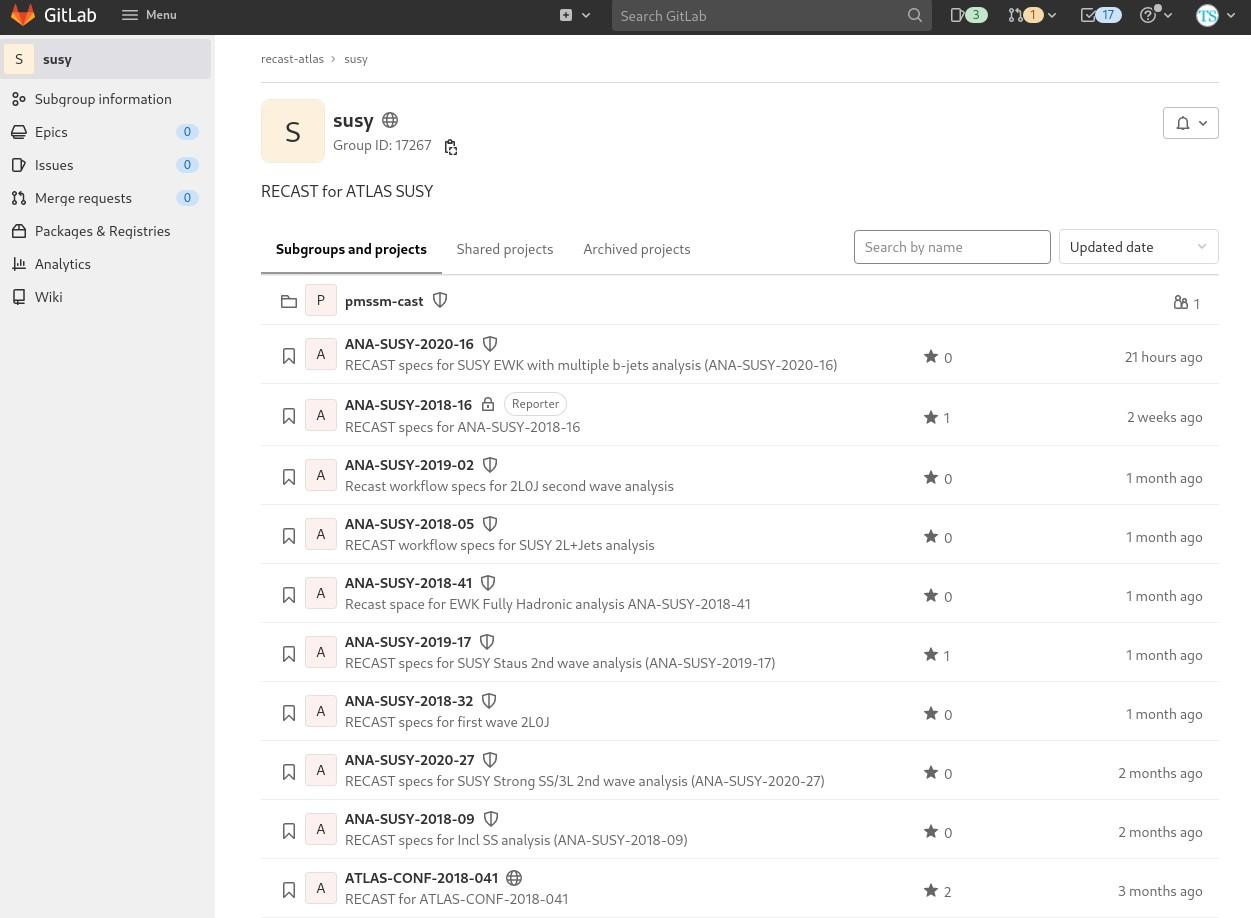
\includegraphics[width=0.9\textwidth]{pmssm-susy-gitlab-repository.png}
\caption{A screenshot of the ATLAS SUSY group analyses preserved on GitLab. Each repository is labeled with the internal ATLAS analysis identifier and contains both workflow files and additional data files needed for the computational processing.}
\label{fig:pmssmgitlab}
\end{figure}

One typical pMSSM computational workflow is presented in Figure~\ref{fig:dag}.
The workflow consists of three time-consuming ntupling steps that process data files and run in parallel.
The workflow ends with a latter fitting steps that run afterwards.
The dependency of steps in the computational graph is rather simple.
The complexity of the problem lies in having to run several thousands of these workflows in order to cover a sufficient number of pMSSM model points.

\begin{figure}
\centering
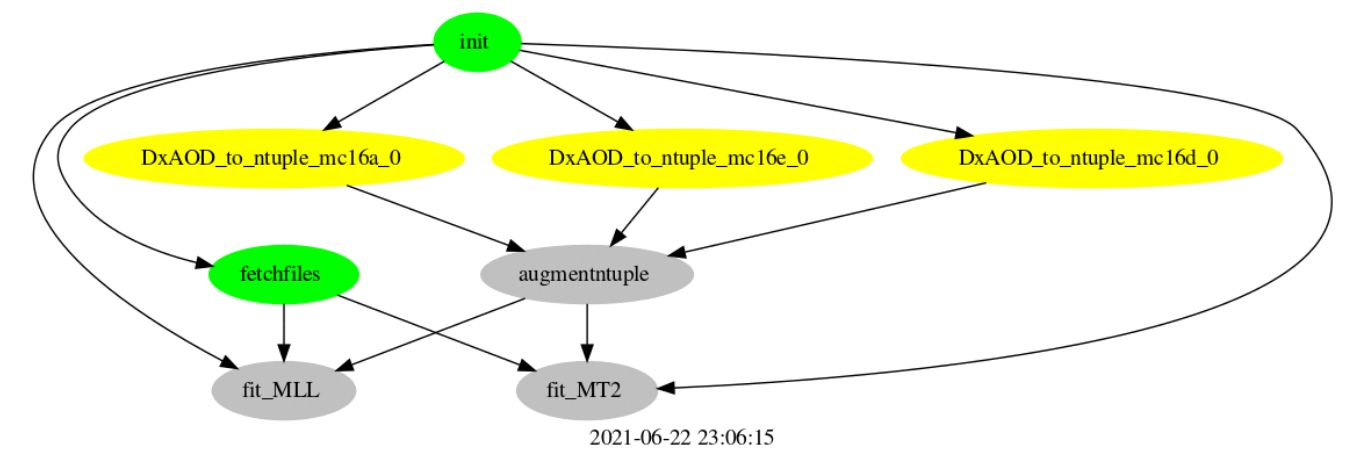
\includegraphics[width=0.9\textwidth, trim=0 40px 0 0, clip]{pmssm-workflow-single.png}
\caption{A typical pMSSM workflow. The computational runtime is about 10 minutes without systematics (test payload) and about 10 hours with all systematics (real payload).}
\label{fig:dag}
\end{figure}

It was the goal of the present work to study the feasibility of running several thousands of these containerised workflows in parallel in an automated way in order to facilitate typical pMSSM studies.
